% vim: spell spelllang=pt formatoptions+=tcwa textwidth=98 nonu foldcolumn=0
% vim: ts=4 sw=4 sts=4 expandtab
\documentclass{beamer}
\usepackage[brazil]{babel}
\usepackage[utf8]{inputenc}
\usepackage[T1]{fontenc}
\usepackage{graphicx,epstopdf,wrapfig,caption,url}

\title[MIHS]{Media Independent Handover Services}
\author{Higor Eurípedes P. F. A.}
\institute[IFTO]{Instituto Federal de Educação, Ciência e Tecnologia do Tocantins}
\date[Dezembro 2011]{23 Dezembro 2011}

\AtBeginSection[]
{
  \begin{frame}
    \frametitle{Media Independent Handover Services}
    \tableofcontents[currentsection,currentsubsection]
  \end{frame}
}
\AtBeginSubsection[]
{
  \begin{frame}
    \frametitle{Media Independent Handover Services}
    \tableofcontents[currentsection,currentsubsection]
  \end{frame}
}

\usetheme{default}
\usecolortheme{seahorse}

\begin{document}
    \frame{\titlepage}

    \frame{
        \frametitle{Apresentação}
        \tableofcontents
    }

    \section{Objeto de estudo}

    \frame{
        \frametitle{\insertsectionhead}

        \begin{itemize}

            \item IEEE 802.21.
            \item Implementação.
            \item Implantação em sistema provedor de acesso.

        \end{itemize}
    }

    \section{O padrão IEEE 802.21}

    \frame{
        \frametitle{\insertsectionhead}
        \framesubtitle{Muito prazer, meu nome é MIHS}

        \begin{block}{O que é?}
            \begin{itemize}

                \item Facilitador de transições entre redes heterogêneas.
                \item Abstração das camadas de enlace e rede.
                \item Fornece uma função para \textit{handover} independente 
                do meio físico.

            \end{itemize}
        \end{block}
        
        \begin{block}{Porquê?}
            \begin{enumerate}

                \item Mobilidade se tornou tendência.
                \item Interesse de WGs de padrões sem fio.
                \item Agregar e desenvolver conceitos comuns.
                \item Otimizar o uso dos recursos.

            \end{enumerate}
        \end{block}

    }
    
    \frame{
        \frametitle{\insertsectionhead}
        \framesubtitle{Era uma vez...}
        \begin{block}{Quando?}
            \begin{itemize}

                \item Novembro, 2002 -- Organização do tutorial de 
                \textit{IEEE 802 handover} para janeiro de 2003.
                \item Janeiro, 2003 -- Apresentação do tutorial.
                \item Fevereiro, 2003 -- Discussões gerais sobre a criação de 
                um \textit{work group} (WG) para o assunto.
                \item Março, 2003 -- Iniciam as reuniões para a criação do WG.
                \item Novembro, 2003 -- WG aprovado.
                \item Março, 2004 -- Reunião inicial do WG.
                \item Maio, 2005 -- Publicação do primeiro \textit{draft}.
                \item Janeiro, 2009 -- Publicação do padrão.

            \end{itemize}
        \end{block}
    }

    \frame{
        \frametitle{\insertsectionhead}
        \framesubtitle{Exemplo de transição}
        \begin{figure}
            \includegraphics[width=\textwidth]{apresentacao-dez-2011/visaogeral.eps}
        \end{figure}
    }

    \subsection{A Media Independent Handover Function (MIHF)}

    \frame{
        \frametitle{\insertsubsectionhead}
       
        \begin{columns}[c]
        \column{.7\textwidth}

        \begin{block}{O que é e o que faz?}
            \begin{itemize}

                \item É uma entidade lógica.
                \item Está posicionada entre as camadas 2 e 3.
                \item Abstrai camadas inferiores por meio de serviços:

                \begin{itemize}

                    \item Media Independent Information Service.
                    \item Media Independent Event Service.
                    \item Media Independent Command Service.

                \end{itemize}

                \item Pode se comunicar com outras MIHF.

            \end{itemize}

        \end{block}

        \column{.3\textwidth}
        \begin{figure}
            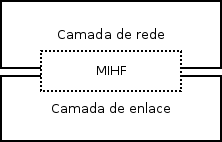
\includegraphics[width=\textwidth]{apresentacao-dez-2011/posicionamento.eps}
        \end{figure}
        \begin{figure}
            \includegraphics[width=\textwidth]{apresentacao-dez-2011/servicos.eps}
        \end{figure}
        \end{columns}
    }

    \frame{
        \frametitle{\insertsubsectionhead}
        \framesubtitle{Service Access Points}

        \begin{columns}[c]

        \column{.6\textwidth}
        \begin{block}{Interação}

            Realizada através de Service Access Points (SAP):
            
            \begin{itemize}

                \item MIH\_Sap
                \item MIH\_Link\_Sap
                
            \end{itemize}
            
        \end{block}
        \column{.4\textwidth}
        \begin{figure}
            \includegraphics[width=\textwidth]{apresentacao-dez-2011/relacaosap.eps}
        \end{figure}
        \end{columns}

    }
    

    
    \frame{
        \frametitle{\insertsubsectionhead}
        \framesubtitle{Media Independent Event Service (MIES)}

        \begin{columns}[c]

        \column{.7\textwidth}
        \begin{block}{Visão geral}
            \begin{itemize}
                
                \item Responsável pela propagação de eventos.
                \item Possui duas categorias de eventos: de enlace e 
                independente do meio (MIH).
                \item Trabalha sob regime de inscrição.

            \end{itemize}
        \end{block}
        
        \column{.3\textwidth}
        \begin{figure}
            \includegraphics[width=\textwidth]{apresentacao-dez-2011/classeventos.eps}
        \end{figure}

        \end{columns}
    }
    
    \frame{
        \frametitle{\insertsubsectionhead}
        \framesubtitle{Media Independent Event Service (MIES)}
        \begin{figure}
            \includegraphics[width=\textwidth]{apresentacao-dez-2011/seq-eventos.eps}
        \end{figure}
    }
    
    \frame{
        \frametitle{\insertsubsectionhead}
        \framesubtitle{Media Independent Event Service (MIES)}
        \begin{figure}
            \includegraphics[width=\textwidth]{apresentacao-dez-2011/eventoremoto.eps}
        \end{figure}
    }
    
    \frame{
        \frametitle{\insertsubsectionhead}
        \framesubtitle{Media Independent Event Service (MIES)}

        \begin{table}[h]
        \caption{Eventos de Enlace}

        \resizebox{\textwidth}{!}{

            \begin{tabular}[b]{ | l | l | }
            \hline
            Link\_Detected            & Novo link foi detectado.          \\
            \hline
            Link\_Up                  & Enlace estabelecido.              \\
            \hline
            Link\_Down                & Enlace quebrado.                  \\
            \hline
            Link\_Parameters\_Report   & Limite de qualidade ultrapassado. \\
            \hline
            Link\_Going\_Down          & Condições de acesso degradadas.   \\
            \hline
            Link\_Handover\_Imminent   & Handover acontecerá em breve.     \\
            \hline
            Link\_Handover\_Complete   & Handover finalizado.              \\
            \hline
            Link\_PDU\_Transmit\_Status &                                   \\
            \hline
            \end{tabular}
        }

        \end{table}
    }
    
    \frame{
        \frametitle{\insertsubsectionhead}
        \framesubtitle{Media Independent Event Service (MIES)}

        \begin{table}[h]
        \caption{Eventos MIH}

        \resizebox{\textwidth}{!}{

            \begin{tabular}[b]{ | l | l | }
            \hline
            MIH\_Link\_Detected            & Novo link foi detectado.          \\
            \hline
            MIH\_Link\_Up                  & Enlace estabelecido.              \\
            \hline
            MIH\_Link\_Down                & Enlace quebrado.                  \\
            \hline
            MIH\_Link\_Parameters\_Report   & Limite de qualidade ultrapassado. \\
            \hline
            MIH\_Link\_Going\_Down          & Condições de acesso degradadas.   \\
            \hline
            MIH\_Link\_Handover\_Imminent   & Handover acontecerá em breve.     \\
            \hline
            MIH\_Link\_Handover\_Complete   & Handover finalizado.              \\
            \hline
            MIH\_Link\_PDU\_Transmit\_Status &                                   \\
            \hline
            \end{tabular}
        }

        \end{table}
    }
    
    \frame{
        \frametitle{\insertsubsectionhead}
        \framesubtitle{Media Independent Command Service (MICS)}

        \begin{columns}[c]

        \column{.7\textwidth}
        \begin{block}{Visão geral}
            \begin{itemize}
                
                \item Fornece meios para interação com camadas inferiores.
                \item Possui duas categorias de eventos: de enlace e 
                independente do meio (MIH).

            \end{itemize}
        \end{block}
        
        \column{.3\textwidth}
        \begin{figure}
            \includegraphics[width=\textwidth]{apresentacao-dez-2011/classcomandos.eps}
        \end{figure}

        \end{columns}
    }
    
    \frame{
        \frametitle{\insertsubsectionhead}
        \framesubtitle{Media Independent Command Service (MICS)}
        \begin{figure}
            \includegraphics[width=\textwidth]{apresentacao-dez-2011/comandoremoto.eps}
        \end{figure}
    }

    \frame{
        \frametitle{\insertsubsectionhead}
        \framesubtitle{Media Independent Command Service (MICS)}

        \begin{table}[h]
        \caption{Comandos de Enlace}

        \resizebox{\textwidth}{!}{
            \begin{tabular}[b]{ | l | l | }
            \hline
            Link\_Capability\_Discover  & Obtem lista de comandos e eventos de enlace. \\
            \hline
            Link\_Event\_Subscribe      & Inscrição.                                   \\
            \hline
            Link\_Event\_Unsubscribe    & Cancelamento de inscrição.                   \\
            \hline
            Link\_Get\_Parameters       & Obtem o estado do enlace.                    \\
            \hline
            Link\_Configure\_Thresholds & Altera comportamento do Link\_Parameters\_Report \\
            \hline
            Link\_Action                & Requisita uma ação ao enlace.            \\
            \hline

            \end{tabular}
        }

        \end{table}
    }
    \frame{
        \frametitle{\insertsubsectionhead}
        \framesubtitle{Media Independent Command Service (MICS)}

        \begin{table}[h]
        \caption{Comandos MIH}

        \resizebox{\textwidth}{!}{
            \begin{tabular}[b]{ | l | l | l | }
            \hline
            MIH\_Link\_Get\_Parameters       & L, R & Obtem o estado do enlace..                           \\
            \hline
            MIH\_Link\_Configure\_Thresholds & L, R & Altera o comportamento do MIH\_Link\_Parameters\_Report \\
            \hline
            MIH\_Link\_Actions              & L, R & Requisita uma ação ao enlace.                        \\
            \hline
            MIH\_Net\_HO\_Candidate\_Query    & R    & Iniciar handover e enviar redes sugeridas.           \\
            \hline
            MIH\_MN\_HO\_Candidate\_Query     & R    & Solicitar sugestões de redes.                        \\
            \hline
            MIH\_N2N\_HO\_Query\_Resources    & R    & Solicita informações de um servidor MIHF             \\
            \hline
            MIH\_MN\_HO\_Commit              & R    & Informa ao servidor atual o servidor-destino.        \\
            \hline
            MIH\_Net\_HO\_Commit             & R    & Informa ao cliente o servidor-destino.               \\
            \hline
            MIH\_N2N\_HO\_Commit             & R    & Informa ao servidor-destino sobre o cliente.         \\
            \hline
            MIH\_MN\_HO\_Complete            & R    & Informa ao servidor-destino o estado do \textit{handover}. \\
            \hline
            MIH\_N2N\_HO\_Complete           & R    & Informa aos servidores o estado do \textit{handover}. \\
            \hline

            \end{tabular}
        }
        \end{table}
    }

    \frame{
        \frametitle{\insertsubsectionhead}
        \framesubtitle{Media Independent Command Service (MICS)}

        \begin{block}{Procedimento simplificado de \textit{handover}}

            \begin{figure}
                \includegraphics[width=\textwidth]{apresentacao-dez-2011/handoversimplificado.eps}
            \end{figure}

        \end{block}
    }
    
    
    \frame{
        \frametitle{\insertsubsectionhead}
        \framesubtitle{Media Independent Information Service (MIIS)}

        \begin{block}{Visão geral}
            \begin{itemize}

                \item Responsável por coletar e fornecer informações sobre o 
                estado das redes.
                \item Possui dois modos de operação: \textit{pull} e 
                \textit{push}.
                \item Também pode trabalhar com informações sobre os MNs.*

            \end{itemize}
        \end{block}
    }

    \frame{
        \frametitle{ODTONE}

        \begin{block}{Demonstração}
            
        \end{block}
    }

\end{document}

